% Do not compile this file directly. It is included by main.tex
% Preamble.tex
% !TeX root = raytracing/slides/main.tex
% raytracing_preamble.tex
% Common styling for Ray Tracing presentation

\documentclass[10pt]{beamer}
\usetheme{metropolis}
\usefonttheme{professionalfonts}

% --- Color Definitions ---
\definecolor{PrimaryColor}{RGB}{33,52,72}         % Deep navy
\definecolor{SecondaryColor}{RGB}{84,119,146}     % Desaturated blue-gray
\definecolor{AccentColor}{RGB}{100, 156, 165}       % Soft steel blue

\definecolor{BackgroundColor}{RGB}{245,247,250}   % Very light cool gray/blue-tinted white
\definecolor{TextColor}{RGB}{40,55,70}            % Darker, cool-toned charcoal (slightly less saturated)
\definecolor{LightGray}{RGB}{220,225,230}         % Soft, cool light gray
\definecolor{DarkGray}{RGB}{70,90,105}            % Cool-toned dark gray (coherent with Primary/Secondary)

\definecolor{RayColor}{RGB}{230,150,80}           % Muted warm orange (less saturated than pure orange)
\definecolor{ObjectColor}{RGB}{128,101,160}       % Muted violet (adjusted purple to match cool palette)
\definecolor{LightColor}{RGB}{235,200,100}        % Soft golden yellow (to complement cool blues)

% --- Theme Customization ---
\setbeamercolor{background canvas}{bg=BackgroundColor}
\setbeamercolor{normal text}{fg=TextColor}
\setbeamercolor{frametitle}{bg=PrimaryColor, fg=white}
\setbeamercolor{section in toc}{fg=PrimaryColor}
\setbeamercolor{block title}{bg=PrimaryColor!80, fg=white}
\setbeamercolor{block body}{bg=PrimaryColor!10}
\setbeamercolor{alerted text}{fg=AccentColor}
\setbeamercolor{itemize item}{fg=PrimaryColor}
\setbeamercolor{itemize subitem}{fg=SecondaryColor}
\setbeamerfont{frametitle}{size=\large,series=\bfseries}

% --- Packages ---
\usepackage[utf8]{inputenc}
\usepackage{url}
\usepackage{booktabs}
\usepackage{amsmath, amssymb}
\usepackage{fontawesome5}
\usepackage{pifont}
\usepackage[most]{tcolorbox}
\tcbuselibrary{skins}
\usepackage{colortbl}
\usepackage{array}
\usepackage{tikz}
\usepackage{graphicx}
\usetikzlibrary{shapes.callouts, positioning, arrows.meta, shapes.geometric, shadows, calc, patterns, 3d, backgrounds, shadings}
\usepackage{adjustbox}
\usepackage{ragged2e}
\usepackage{pgfplots}
\usepackage{graphicx}
\usepackage{caption}
\usepackage{minted}
\pgfplotsset{compat=1.18}

% --- Custom Commands ---
\newcommand{\cmark}{\textcolor{SecondaryColor}{\ding{51}}}
\newcommand{\xmark}{\textcolor{AccentColor}{\ding{55}}}
\newcommand{\highlight}[1]{\textcolor{PrimaryColor}{\textbf{#1}}}
\newcommand{\raycolor}[1]{\textcolor{RayColor}{\textbf{#1}}}
\newcommand{\objectcolor}[1]{\textcolor{ObjectColor}{\textbf{#1}}}

% --- TikZ styles for ray tracing visualizations ---
\tikzstyle{process} = [rectangle, rounded corners=3mm, minimum width=2cm, minimum height=0.8cm, text centered, draw=PrimaryColor, thick, fill=PrimaryColor!15, drop shadow]
\tikzstyle{arrow} = [thick, PrimaryColor, ->, >=stealth]
\tikzstyle{ray} = [thick, RayColor, ->, >=stealth]
\tikzstyle{lightray} = [thick, LightColor, ->, >=stealth]
\tikzstyle{reflectray} = [thick, SecondaryColor, ->, >=stealth]
\tikzstyle{refractray} = [thick, AccentColor, ->, >=stealth]
\tikzstyle{shadowray} = [thick, DarkGray, ->, >=stealth, dashed]

% --- 3D object styles ---
\tikzstyle{sphere} = [circle, minimum size=1.5cm, draw=ObjectColor, thick, fill=ObjectColor!20, drop shadow]
\tikzstyle{plane} = [rectangle, minimum width=3cm, minimum height=0.2cm, draw=ObjectColor, thick, fill=ObjectColor!20]
\tikzstyle{triangle} = [regular polygon, regular polygon sides=3, minimum size=1.5cm, draw=ObjectColor, thick, fill=ObjectColor!20]

% --- Eye/Camera styles ---
\tikzstyle{eye} = [circle, minimum size=0.8cm, draw=PrimaryColor, thick, fill=PrimaryColor!30]
\tikzstyle{pixel} = [rectangle, minimum size=0.2cm, draw=AccentColor, fill=AccentColor!30]

% --- Text box styles ---
\tikzstyle{conceptbox} = [rectangle, rounded corners, fill=PrimaryColor!10, draw=PrimaryColor, thick, text width=0.8\textwidth, inner sep=8pt]
\tikzstyle{formulabox} = [rectangle, rounded corners, fill=SecondaryColor!10, draw=SecondaryColor, thick, inner sep=6pt]

% --- Custom environments ---
\newtcolorbox{raybox}[1]{
  colback=RayColor!10,
  colframe=RayColor,
  title=#1,
  fonttitle=\bfseries,
  sharp corners
}

\newtcolorbox{conceptbox}[1]{
  colback=PrimaryColor!10,
  colframe=PrimaryColor,
  title=#1,
  fonttitle=\bfseries,
  rounded corners
}

\newtcolorbox{mathbox}[1]{
  colback=SecondaryColor!10,
  colframe=SecondaryColor,
  title=#1,
  fonttitle=\bfseries,
  rounded corners
}

\newenvironment{timeline}{%
  \begin{tikzpicture}[scale=0.8]
    \coordinate (start) at (0,0);
    \newcounter{timelineitem}
    \setcounter{timelineitem}{0}
  }{%
  \end{tikzpicture}
}

\newcommand{\timelineitem}[4]{%
  \stepcounter{timelineitem}%
  % Name of this item’s node
  \edef\thisID{time\thetimelineitem}%
  \ifnum\value{timelineitem}=1
  % First item: anchor at (start)
  \node[rectangle, draw, fill=PrimaryColor!20,
  text width=1.5cm, minimum height=0.8cm, align=center]
  (\thisID) at (start) {\textbf{#2}};
  \else
  % Later items: below=#1 of previous time node
  \pgfmathtruncatemacro\prev{\value{timelineitem}-1}%
  \node[rectangle, draw, fill=PrimaryColor!20,
    text width=1.5cm, minimum height=0.8cm, align=center,
  below=#1 of time\prev]
  (\thisID) {\textbf{#2}};
  \fi
  % Description always to the right of this time node
  \node[rectangle, draw, fill=SecondaryColor!10,
    text width=4cm, minimum height=0.8cm,
  align=left, right=0.3cm of \thisID]
  (desc\thetimelineitem) {\textbf{#3}\\#4};
  % Draw arrow back to previous if not the first
  \ifnum\value{timelineitem}>1
  \draw[->, thick, PrimaryColor]
  (time\prev.south) -- (\thisID.north);
  \fi
}

\tikzset{
  camera/.style={fill=PrimaryColor!60, draw=PrimaryColor!80, rectangle, minimum size=8pt},
  image plane/.style={fill=AccentColor!10, draw=AccentColor!50, opacity=0.8},
  pixel/.style={fill=AccentColor!60, thick},
  primary ray/.style={->, very thick, red!90},
  object/.style={fill=ObjectColor!60, draw=ObjectColor!80, circle, minimum size=12pt},
  fovangle/.style={<->, thick, PrimaryColor, dashed}
}

\tikzset{
  lens/.style={thick, PrimaryColor, line width=3pt},
  focal plane/.style={thick, AccentColor},
  object ray/.style={->, thick, ObjectColor},
  image ray/.style={->, thick, SecondaryColor},
  optical axis/.style={dashed, gray}
}

\newcommand{\lens}[3]{%
  \begingroup
  % half‐dimensions
  \pgfmathsetlengthmacro{\a}{#2}%
  \pgfmathsetlengthmacro{\b}{#3}%
  \pgfmathsetlengthmacro{\c}{#3/2}%
  \begin{scope}[shift={#1}]
    \draw[line join=round, fill=blue!15]
    (0,-{\c})
    arc(-30:30:{\a} and {\b})
    arc(150:210:{\a} and {\b})
    ;
  \end{scope}
  \endgroup
}

\title{Signed Distance Fields}
\subtitle{A Modern Approach to Shape Representation in Graphics}
\author{Md. Miraj Hasan (2005084)\\
Wahid Al Azad Navid (2005089)}
\institute{Department of Computer Science and Engineering\\Bangladesh University of Engineering and Technology (BUET)}

\begin{document}

\begin{frame}
  \titlepage
\end{frame}

\begin{frame}{Index}
  \vspace{0.5cm}
  \tiny
  \tableofcontents
\end{frame}

\section{Introduction}
\begin{frame}{What are Signed Distance Fields?}
  \begin{conceptbox}{Definition}
    A \textbf{Signed Distance Field (SDF)} is a function that gives the shortest distance between any point and the surface of a shape.
    \\~\\
    \pause % First pause: show only the definition above
    The sign indicates:
    \begin{itemize}
      \item<2-> Negative: \textit{inside} the shape
      \item<3-> Positive: \textit{outside} the shape
      \item<4-> Zero: \textit{on the surface}
    \end{itemize}
  \end{conceptbox}
\end{frame}

\section{Mathematical Foundation}
\begin{frame}{Mathematical Definition of SDF}
  \begin{mathbox}{Formal Expression}
    \[
      f(\mathbf{x}) = \pm \min_{\mathbf{p} \in \partial \Omega} \|\mathbf{x} - \mathbf{p}\|
    \]
    \pause
    \begin{itemize}[<+->]
      \item $\mathbf{x}$ = arbitrary point
      \item $\partial \Omega$ = surface boundary
      \item $f(\mathbf{x}) < 0$ if inside, $> 0$ if outside
    \end{itemize}
  \end{mathbox}
\end{frame}


\section{Applications}
\begin{frame}{Where are SDFs Used?}
  \begin{itemize}
    \item Real-time rendering and raymarching
    \item Font rendering and anti-aliasing
    \item Collision detection and physics
    \item Procedural modeling and morphing
    \item Implicit surfaces and shape blending
  \end{itemize}
\end{frame}

\section{Basic Shapes as SDFs}
\begin{frame}{SDFs for Primitive Shapes}
  \begin{itemize}
    \item \textbf{Sphere:} $f(\mathbf{x}) = \|\mathbf{x} - \mathbf{c}\| - r$
    \item \textbf{Box:} Uses component-wise signed distance
    \item \textbf{Plane, Torus, etc.}: Custom distance functions
  \end{itemize}
  \begin{conceptbox}{Key Benefit}
    Complex shapes can be formed using simple operations like union, intersection, and subtraction.
  \end{conceptbox}
\end{frame}

\section{SDF Raymarching}
\begin{frame}{Raymarching with SDFs}
  \begin{conceptbox}{Algorithm}
    \begin{enumerate}
      \item<1-> Cast a ray from the eye
      \item<2-> At each step, query the SDF to get the distance to the closest object
      \item<3-> Advance along the ray by that distance
      \item<4-> Stop when distance $< \varepsilon$ (or max steps)
    \end{enumerate}
  \end{conceptbox}
\end{frame}

\begin{frame}{Raymarching with Multiple Objects}
  \centering
  \vspace{0.5cm}
  % No \only<5-> here. Let the picture’s own <1->, <2->… drive the animation.
  \resizebox{0.8\linewidth}{!}{% raymarching_diagram.tex  (NO \begin{frame} ... \end{frame} here)
\begin{tikzpicture}[scale=1]
  % Camera
  \node[eye] (eye) at (0,0) {\faIcon{eye}};

  % Ray path
  \draw[ray] (eye) -- (7,0);

  % --- Objects (two SDF shapes) ---
  \node[sphere, fill=ObjectColor!35, minimum size=1.0cm] at (3.6,1.0) {};
  \node[above right] at (4.1,0.6) {\tiny \objectcolor{Object A}};

  \node[sphere, fill=ObjectColor!40, minimum size=2.0cm] at (6.5,0.0) {};
  \node[below] at (6.5,-1.0) {\footnotesize \objectcolor{Object B}};

  % --- March steps (appear one by one) ---
  \onslide<1->{\draw[AccentColor, thick, dashed] (1.6,0) circle (1.6);}  % r1
  \onslide<2->{\draw[AccentColor, thick, dashed] (3.2,0) circle (0.25);}  % r2
  \onslide<3->{\draw[AccentColor, thick, dashed] (3.45,0) circle (0.18);} % r3
  \onslide<4->{\draw[AccentColor, thick, dashed] (3.63,0) circle (0.12);} % r4
  \onslide<5->{\draw[AccentColor, thick, dashed] (3.75,0) circle (0.90);} % r5
  \onslide<6->{\draw[AccentColor, thick, dashed] (4.65,0) circle (0.60);} % r6
  \onslide<7->{\draw[AccentColor, thick, dashed] (5.25,0) circle (0.30);} % r7

\end{tikzpicture}
}
\end{frame}





\section{Font Rendering}
\begin{frame}{High-Quality Fonts with SDFs}
  \begin{columns}
    \begin{column}{0.6\textwidth}
      \begin{conceptbox}{Valve's Technique}
        \begin{itemize}
          \item Glyphs stored as SDFs in textures
          \item Smooth scaling and edge rendering
          \item Great for HUDs and UIs in games
        \end{itemize}
      \end{conceptbox}
    \end{column}
    \begin{column}{0.4\textwidth}
      \centering
      \resizebox{\linewidth}{!}{
        \begin{tikzpicture}[scale=1.2]
  % Pixel grid background
  \foreach \x in {0,...,5} {
    \foreach \y in {0,...,4} {
      \pgfmathsetmacro{\val}{int(100 - abs(\x-2.5)*30 - abs(\y-2)*30)}
      \fill[gray!\val!white] (\x,-\y) rectangle ++(1,-1);
    }
  }

  % Outline of glyph "A"
  \draw[PrimaryColor, ultra thick] (1,-1) -- (2.5,-4) -- (4,-1);
  \draw[PrimaryColor, ultra thick] (1.8,-2.5) -- (3.2,-2.5);

  \node[above] at (2.5,0.5) {\small SDF Texture for Letter A};
\end{tikzpicture}

      }
    \end{column}
  \end{columns}
\end{frame}

\section{Collision Detection}
\begin{frame}{Collision Detection with SDFs}
  \begin{conceptbox}{Key Idea}
    The signed distance tells how far one object is from another. 
    If the value is negative, it means collision.
  \end{conceptbox}

  \begin{itemize}
    \item<1-> Efficient for character and object physics
    \item<2-> Simple penetration depth calculation
    \item<3-> Used in soft-body and rigid-body physics engines
  \end{itemize}

  \vspace{0.5cm}
  \centering
  \only<4->{\resizebox{0.4\linewidth}{!}{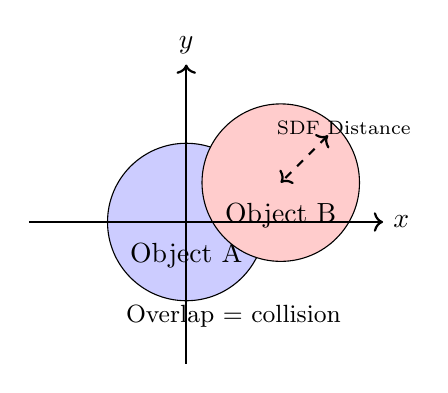
\begin{tikzpicture}
  \draw[fill=blue!20] (0,0) circle (1) node[below=4pt] {Object A};
  \draw[fill=red!20] (1.2,0.5) circle (1) node[below=4pt] {Object B};

  \draw[->, thick] (-2, 0) -- (2.5, 0) node[right] {$x$};
  \draw[->, thick] (0, -1.8) -- (0, 2) node[above] {$y$};

  \node at (0.6, -1.2) {\small Overlap = collision};
  \draw[<->, dashed, thick] (1.8,1.1) -- (1.2,0.5);
  \node at (2,1.2) {\scriptsize SDF Distance};
\end{tikzpicture}
}}
\end{frame}



\section{Procedural Modeling}
\begin{frame}{Procedural Modeling and Morphing}
  \begin{conceptbox}{Using SDF Operations}
    You can build complex models using:
    \begin{itemize}
      \item \texttt{Union}: $f = \min(f_1, f_2)$
      \item \texttt{Intersection}: $f = \max(f_1, f_2)$
      \item \texttt{Difference}: $f = \max(f_1, -f_2)$
    \end{itemize}
  \end{conceptbox}

  \vspace{0.3cm}
  \centering
  \resizebox{0.75\linewidth}{!}{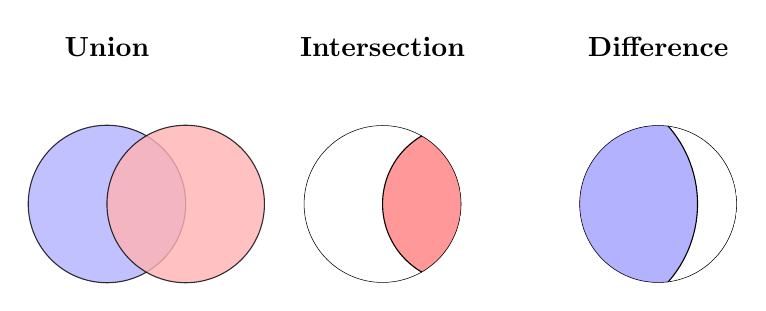
\begin{tikzpicture}
  % Labels
  \node at (-3.5,2) {\textbf{Union}};
  \node at (0,2)     {\textbf{Intersection}};
  \node at (3.5,2)   {\textbf{Difference}};

  % Union
  \begin{scope}[shift={(-3.5,0)}]
    \draw[fill=blue!30,opacity=0.8] (0,0) circle (1);
    \draw[fill=red!30,opacity=0.8] (1,0) circle (1);
  \end{scope}

  % Intersection
  \begin{scope}[shift={(0,0)}]
    \clip (0,0) circle (1);
    \fill[red!40] (1,0) circle (1);
    \draw (0,0) circle (1);
    \draw (1,0) circle (1);
  \end{scope}

  % Difference
  \begin{scope}[shift={(3.5,0)}]
    \clip (0,0) circle (1);
    \fill[blue!30] (-1,0) circle (1.5);
    \draw (0,0) circle (1);
    \draw (-1,0) circle (1.5);
  \end{scope}
\end{tikzpicture}
}
\end{frame}

\section{Shape Blending}
\begin{frame}{Implicit Surfaces and Blending}
  \begin{conceptbox}{Smooth Transitions}
    \only<1->{SDFs allow smooth blending between shapes using interpolation:}
    \only<2->{\[
      f(x) = \text{lerp}(f_1(x), f_2(x), \alpha)
    \]}
    \only<3->{or soft union: \[
      f = -\log(e^{-k f_1} + e^{-k f_2})/k
    \]}
  \end{conceptbox}

  \vspace{0.3cm}
  \centering
  \only<4->{\resizebox{0.75\linewidth}{!}{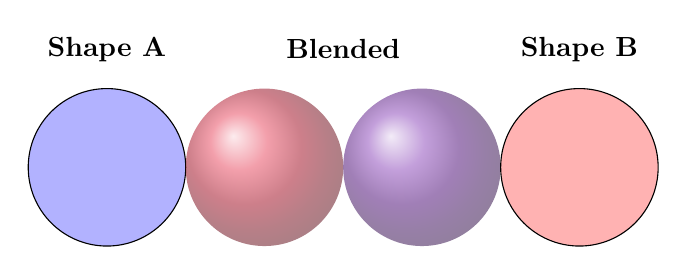
\begin{tikzpicture}
  % Left shape
  \begin{scope}[shift={(-3,0)}]
    \node at (0,1.5) {\textbf{Shape A}};
    \draw[fill=blue!30] (0,0) circle (1);
  \end{scope}

  % Right shape
  \begin{scope}[shift={(3,0)}]
    \node at (0,1.5) {\textbf{Shape B}};
    \draw[fill=red!30] (0,0) circle (1);
  \end{scope}

  % Blended shape
  \begin{scope}[shift={(0,0)}]
    \node at (0,1.5) {\textbf{Blended}};
    \shade[ball color=purple!50!red, opacity=0.5] (-1,0) circle (1);
    \shade[ball color=purple!50!blue, opacity=0.5] (1,0) circle (1);
  \end{scope}
\end{tikzpicture}
}}
\end{frame}




\section{Generating SDFs}
\begin{frame}{How are SDFs Generated?}
  \begin{itemize}
    \item \textbf{Analytical}: Direct formulas for simple shapes
    \item \textbf{Voxel-based}: Grids for complex models
    \item \textbf{From images}: Euclidean distance transform
    \item \textbf{GPU-based}: Jump Flood Algorithm (JFA)
  \end{itemize}
\end{frame}

\section{Modern Extensions}
\begin{frame}{Recent Innovations}
  \begin{itemize}
    \item \textbf{Neural SDFs}: Learnable representations (e.g., NeRF)
    \item \textbf{Volumetric rendering}: Clouds, fog, soft shadows
    \item \textbf{SDF octrees}: Efficient memory and level-of-detail
  \end{itemize}
\end{frame}

\section{Conclusion}
\begin{frame}{Conclusion}
  \begin{conceptbox}{Key Takeaways}
    \begin{itemize}
      \item Compact, efficient way to represent shapes
      \item Ideal for GPU and real-time applications
      \item Extensible to AI, physics, VFX, and more
    \end{itemize}
  \end{conceptbox}
\end{frame}

\end{document}
